\documentclass[11pt]{article}

% parameters are fairly self-explanatory here, thankfully
\usepackage[width=7in,height=9.5in,top=0.75in,centering]{geometry}

% for math-ing
\usepackage{amsmath}
\usepackage{amssymb}
\usepackage{comment}
\usepackage{graphicx}
%%%%%% tables %%%%%%%%

\usepackage{array}
\renewcommand{\arraystretch}{1.5}
\setlength{\tabcolsep}{8pt}

%%%%%% plotting %%%%%%

\usepackage[dvipsnames]{xcolor}
\usepackage{tikz}
\usepackage{pgfplots}

\pgfplotsset{every axis/.append style={
                    axis x line=middle,    % put the x axis in the middle
                    axis y line=middle,    % put the y axis in the middle
                    axis line style={<->,color=black}, % arrows on the axis
                    xlabel={$x$},          % default put x on x-axis
                    ylabel={$y$},          % default put y on y-axis
            }}
            
 \pgfplotsset{compat=1.14} % sometimes, everything falls apart without this
 
 %\usepgfplotslibrary{fillbetween} %for shading between curves

%%%%%% commands %%%%%%

% exam heading; course name is first argument, exam information is second argument
\newcommand{\Heading}[2]{
    \fbox{
        {\Large\textbf{#1}}
        }
    \hfill
    \fbox{
        \begin{minipage}{0.2\textwidth}
            \begin{center}
            \textbf{#2}
            \end{center}
        \end{minipage}
    }
    \par\vspace{0.1in}}

% for being lazy while beautifying integrals
\newcommand{\dint}{\displaystyle\int}

% for being lazy while beautifying limits
\newcommand{\dlim}{\displaystyle\lim}

%%%%%% stuff %%%%%%

\usepackage{fancyhdr}

%\setcounter{page}{0} % first page is page 0

\parindent0pt % no indent

\fboxsep=0.25cm % little space in fbox border

%%%%%% BEGIN! %%%%%%%

\begin{document}

\pagestyle{fancy}

% record goals here to create sense of transparency

\fancyhead[c]{%
  \ifcase\value{page}
  % empty test for page = 0
  \or {}% 
  \or
  \or {\bf\color{ProcessBlue} F2: Exponentials \& Log Functions}% page=1
  \or {\bf\color{ForestGreen} D2: Compute Derivatives}% page = 2
  \or {\bf\color{ForestGreen} D3: Derivatives of Basic Functions}% page = 3
  \or {\bf\color{RedOrange} A1: Derivatives and Graphing}% page = 4
  \or {\bf\color{RedOrange} A2: Local and Absolute Extreme Values}% page = 5
  \or {\bf\color{RedOrange} A3: Applied Optimization}% page = 7
  \or {\bf\color{Fuchsia} I1: Meaning of an Integral}% page = 6
  \or {\bf\color{Fuchsia} I2: Properties of Definite Integrals}% page = 8
  \or
  \else
  % Empty chead here!
  \fi
}

\thispagestyle{empty} % don't display that this is page 0

\Heading{MATH 1190/1210 Survey of Calculus I}{Knowledge Checkpoint 3\\Spring 2026}

\vspace{0.1in}

\textbf{Name} \hrulefill \, \begin{minipage}{0.16\textwidth}\begin{center}\textbf{UVA ID\\ (e.g. hdj4nd)} \end{center}\end{minipage}\hrulefill\\

\begin{minipage}{0.2\textwidth}\begin{center}\textbf{Course \&\\ Section Number} \end{center}\end{minipage} \hrulefill\,\,\textbf{Date} \hrulefill  \\

\hrulefill
\paragraph*{Course \& Section Numbers:}

{\small
\begin{center}
\begin{tabular}{| c | c | c | c |}
\hline
\begin{minipage}{0.12\textwidth}\centering
1190-100\\
J. Rolf\\
(2:00 PM)
\end{minipage}
&
\begin{minipage}{0.12\textwidth}\centering
1190-200\\
J. Rolf\\
(3:30 PM)
\end{minipage}
&
\begin{minipage}{0.12\textwidth}\centering
1190-300\\
Michael\\
(11 AM)
\end{minipage}
&
\begin{minipage}{0.12\textwidth}\centering
1210-200\\
Susan\\
(9:30 AM)
\end{minipage}
\\ \hline
\begin{minipage}{0.12\textwidth}\centering
1210-300\\
Susan\\
(2 PM)
\end{minipage}
&
\begin{minipage}{0.12\textwidth}\centering
1210-400\\
Holden\\
(12:30 PM)
\end{minipage}
&
\begin{minipage}{0.12\textwidth}\centering
1210-500\\
Susan\\
(3:30 PM)
\end{minipage}
&
\begin{minipage}{0.12\textwidth}\centering
1210-700\\
Aaratrick\\
(2:00 PM)
\end{minipage}
\\ \hline
\begin{minipage}{0.12\textwidth}\centering
1210-800\\
J. Bowling\\
(3:30 PM)
\end{minipage}
&
\begin{minipage}{0.12\textwidth}\centering
1210-900\\
J. Bowling\\
(5 PM)
\end{minipage}
&
\begin{minipage}{0.12\textwidth}\centering
1210-930\\
Vadim\\
(11 AM)
\end{minipage}
\\
\cline{1-3}
\end{tabular}
\end{center}
}


{%\small

\paragraph*{Instructions:}

\begin{itemize}
    
    \item The regular time allowed for completing this assessment is \fbox{$80$} minutes.
    %\item This assessment is out of 50 points.\\
    \item This assessment contains one single-part or multi-part problem for each of the following targets: {\bf\color{ProcessBlue} F2}, {\bf\color{ForestGreen} D2},   {\bf\color{ForestGreen} D3}, {\bf\color{RedOrange} A1}, {\bf\color{RedOrange} A2}, {\bf\color{RedOrange} A3}, {\bf\color{Fuchsia} I1}, {\bf\color{Fuchsia} I2}.
    \item On each problem, you will receive a score of Exceeds Expectations (5), Proficient (4), Almost (3), Developing (2), Emerging (1), or Not Yet (0). {\bf Please do not interpret your score as a percentage.}
    %\item You will have opportunities to reassess on the targets appearing on this assessment after the next {\bf 2} assessments.\\
    \item You may NOT use calculators, dictionaries, notes, phones, or any other kind of aid.
    \item Please write neatly. What cannot be read, cannot be graded.
    \item Carefully work out each problem and clearly indicate your final answer to every problem.
    \item Throughout, give the most descriptive answer possible. \textbf{For instance, ``DNE" will not be accepted when ``$=\infty$" is applicable.}
    %\item Please provide the most specific answer possible. For instance, if a limit does not exist because it goes to $\infty$ or $-\infty$, then specify this.
    \item Please use the methods discussed up to this point in the course. For example, any work based on l'H\^opital's Rule will not receive credit.
    \item \textbf{All work must be shown unless otherwise specified.} Partial credit will not be given if appropriate work is not shown.
    \item In particular, {\bf any answer appearing with no justification will receive no credit regardless of whether the answer was correct}, unless otherwise specified.
    \item Please first respond to the prompts on which you feel most proficient, then respond to others later.
    \item This booklet is printed double-sided. It contains 12 pages and 8 numbered problems.
    \end{itemize}
    
    }

\vfill


%%%%%%%%%
\newpage

This page is left blank intentionally.\\

Use this page if you need additional space to write your solutions to any problem. \\

If you wish this page graded, you must refer to this page on \textbf{the original page} of the problem. Otherwise, your grader will NOT consider your work on this page.

\newpage%
%%%%%%%%%


\begin{enumerate}

%%%%%%%%%%%%%%%%%%%%%%%%%%%%%%%%%%%%%%%%%%%%%%%%%%%%%
%%%%%%%%%%% BEGIN PROBLEM F2 %%%%%%%%%%%%%%%%%%%%%%%%
%%%%%%%%%%%%%%%%%%%%%%%%%%%%%%%%%%%%%%%%%%%%%%%%%%%%%

\item Respond to the prompts below. In part (a) only, you may simply write your answers.
\begin{itemize}
\item[(a)] Solve the following equation for $x$:
$$2^{2x - 1} = 8$$
\vspace{4cm}


\item[(b)] Use properties of exponents to simplify the following expression. 

\[
\frac{4^{-1}x^5\sqrt{y^3}}{x^{-1/2} \cdot y^2}
\]
\vspace{4cm}

\item[(c)] Given that $\log_2(3) = a$ and $\log_2(5) = b.$ Find the following (Note: Your final answer should be in terms of $a$ and $b$):
\begin{enumerate}
\item $\log_2(15)$\\
\vspace{4cm}

\item $\log_2\left(\dfrac{3}{5}\right)$\\

\end{enumerate}

\end{itemize}


%%%%%%%%%%%%%%%%%%%%%%%%%%%%%%%%%%%%%%%%%%%%%%%%%%%%%
%%%%%%%%%%% END PROBLEM F2 %%%%%%%%%%%%%%%%%%%%%%%%%%
%%%%%%%%%%%%%%%%%%%%%%%%%%%%%%%%%%%%%%%%%%%%%%%%%%%%%

\newpage

%%%%%%%%%%%%%%%%%%%%%%%%%%%%%%%%%%%%%%%%%%%%%%%%%%%%%
%%%%%%%%%%% BEGIN PROBLEM D3 %%%%%%%%%%%%%%%%%%%%%%%%
%%%%%%%%%%%%%%%%%%%%%%%%%%%%%%%%%%%%%%%%%%%%%%%%%%%%%

\item Write down the derivatives of the following functions. 

Although no work is required, you are highly encouraged to include any work that shows your thought process. 

\begin{center}
        \begin{tabular}{l c r l c r}
            %
            $\displaystyle\frac{d}{dx}\left[ \log_{2}(7) + x\right]$ & $=$ & \rule[-8pt]{1.5in}{0.4pt} &
            \vspace{3cm} 

            %$\displaystyle\frac{d}{dx}\left[ 5x^3 \right]$ & $=$ & \rule[-8pt]{1.5in}{0.4pt}\\[0.3in]
            %%%%%
            %$\displaystyle\frac{d}{dx}\left[ \dfrac{4}{x^4} \right]$ & $=$ & \rule[-8pt]{1.5in}{0.4pt} & 
            %%%%%
            $\displaystyle\frac{d}{dx}\left[ e^x-\dfrac{1}{x^2} \right]$ & $=$ & \rule[-8pt]{1.5in}{0.4pt}\\[1in]
            \vspace{3cm} 

            %%%%%
            $\displaystyle\frac{d}{dx}\left[ \log_7(x) \right]$ & $=$ & \rule[-8pt]{1.5in}{0.4pt}&
            %
            $\displaystyle\frac{d}{dx}\left[ \left(\dfrac{5}{7}\right)^x \right]$ & $=$ & \rule[-8pt]{1.5in}{0.4pt}\\[1in]
            %%%%%
            \vspace{3cm} 

            $\displaystyle\frac{d}{dx}\left[ \dfrac{x^8-10x^2 - 3x}{x^2} \right]$ & $=$ & \rule[-8pt]{1.5in}{0.4pt} & 
            %
            $\displaystyle\frac{d}{dx}\left[ 6\sqrt{x^4}-e^1 \right]$ & $=$ & \rule[-8pt]{1.5in}{0.4pt}\\[0.3in]
            %%%%%
        \end{tabular}
        
\end{center}

%%%%%%%%%%%%%%%%%%%%%%%%%%%%%%%%%%%%%%%%%%%%%%%%%%%%%
%%%%%%%%%%% END PROBLEM D3 %%%%%%%%%%%%%%%%%%%%%%%%%%
%%%%%%%%%%%%%%%%%%%%%%%%%%%%%%%%%%%%%%%%%%%%%%%%%%%%%

\newpage

%%%%%%%%%%%%%%%%%%%%%%%%%%%%%%%%%%%%%%%%%%%%%%%%%%%%%
%%%%%%%%%%% BEGIN PROBLEM D2 %%%%%%%%%%%%%%%%%%%%%%%%
%%%%%%%%%%%%%%%%%%%%%%%%%%%%%%%%%%%%%%%%%%%%%%%%%%%%%

\item Find the derivative of the following expressions. 

Write down the steps so that you will be able to receive partial credit if your final answer is not fully correct. There's no need to simplify your final answer.

\begin{enumerate}
\item $f(x) = \dfrac{x \ln(x) + x}{e^x}$

\vfill

\item $g(x) = \sqrt{e^{5x^2}-5}$

\vfill 
\end{enumerate}


%%%%%%%%%%%%%%%%%%%%%%%%%%%%%%%%%%%%%%%%%%%%%%%%%%%%%
%%%%%%%%%%% END PROBLEM D2 %%%%%%%%%%%%%%%%%%%%%%%%%%
%%%%%%%%%%%%%%%%%%%%%%%%%%%%%%%%%%%%%%%%%%%%%%%%%%%%%

\newpage

%%%%%%%%%%%%%%%%%%%%%%%%%%%%%%%%%%%%%%%%%%%%%%%%%%%%%
%%%%%%%%%%% BEGIN PROBLEM A1 %%%%%%%%%%%%%%%%%%%%%%%%
%%%%%%%%%%%%%%%%%%%%%%%%%%%%%%%%%%%%%%%%%%%%%%%%%%%%%

\item Consider the following function:
$f(x) = \dfrac{x^4}{4} - \dfrac{x^2}{2} + 1$
%\begin{center}
%    
\includegraphics[scale=0.4]{KC3A1}
%\end{center}

Answer the following questions. 

\begin{enumerate}
    \item At what $x$-values does $f(x)$ have its critical numbers?
\vspace{3cm}

    {\large
        \[\text{Critical numbers: } \rule[-8pt]{4in}{0.4pt}\]
    }
    \item On what interval(s) is $f(x)$ increasing? On what interval(s) is $f(x)$ decreasing?

\vspace{3cm}

    {\large
        \[\text{Increasing: } \rule[-8pt]{4in}{0.4pt}\]
    }

    {\large
        \[\text{Decreasing: } \rule[-8pt]{4in}{0.4pt}\]
    }

    \item On what interval(s) is $f(x)$ concave up? On what interval(s) is $f(x)$ concave down?
\vspace{3cm}


    {\large
        \[\text{Concave up: } \rule[-8pt]{4in}{0.4pt}\]
    }

    {\large
        \[\text{Concave down: } \rule[-8pt]{4in}{0.4pt}\]
    }



    \item At what $x$-values does $f(x)$ have its inflection points?
\vspace{3cm}


    {\large
        \[\text{Inflection points ($x$-value(s) only): } \rule[-8pt]{3in}{0.4pt}\]
    }
\end{enumerate}

%%%%%%%%%%%%%%%%%%%%%%%%%%%%%%%%%%%%%%%%%%%%%%%%%%%%%
%%%%%%%%%%% END PROBLEM A1 %%%%%%%%%%%%%%%%%%%%%%%%%%
%%%%%%%%%%%%%%%%%%%%%%%%%%%%%%%%%%%%%%%%%%%%%%%%%%%%%

\newpage

%%%%%%%%%%%%%%%%%%%%%%%%%%%%%%%%%%%%%%%%%%%%%%%%%%%%%
%%%%%%%%%%% BEGIN PROBLEM A2 %%%%%%%%%%%%%%%%%%%%%%%%
%%%%%%%%%%%%%%%%%%%%%%%%%%%%%%%%%%%%%%%%%%%%%%%%%%%%%

\item Let 
\[
f(x) = (x - 2)^{4/3}
\]

You may take as given that
\[
f'(x) = \frac{4}{3}(x - 2)^{1/3} , \quad \text{and} \quad f''(x) = \frac{4}{9(x-2)^{2/3}}.
\]

\begin{enumerate}

\item[(a)] Find all critical numbers of $f$.

\vspace{4cm}

\item[(b)] What does the First Derivative Test tell us about the behavior of $f$ at its critical numbers?  
You must show sign analysis to receive full credit.

\vspace{4cm}

\item[(c)] What does the Second Derivative Test tell us about the behavior of $f$ at its critical numbers?  

\vspace{4cm}

\item[(d)] On the interval $[0,3]$, determine where $f$ attains its absolute maximum and absolute minimum values. Clearly justify your answer.

\end{enumerate}


%%%%%%%%%%%%%%%%%%%%%%%%%%%%%%%%%%%%%%%%%%%%%%%%%%%%%
%%%%%%%%%%% END PROBLEM A2 %%%%%%%%%%%%%%%%%%%%%%%%%%
%%%%%%%%%%%%%%%%%%%%%%%%%%%%%%%%%%%%%%%%%%%%%%%%%%%%%

\newpage

%%%%%%%%%%%%%%%%%%%%%%%%%%%%%%%%%%%%%%%%%%%%%%%%%%%%%
%%%%%%%%%%% BEGIN PROBLEM A3 %%%%%%%%%%%%%%%%%%%%%%%%
%%%%%%%%%%%%%%%%%%%%%%%%%%%%%%%%%%%%%%%%%%%%%%%%%%%%%

\item A Norman window has the shape of a rectangle with height $y$ surmounted by a semicircle with radius $x$ (see the accompanying figure). If a Norman window is to have a perimeter of (4 + $\pi$) ft, what should its dimensions be in order to allow the maximum area of light through the window?


\begin{figure}[h]
    \centering
    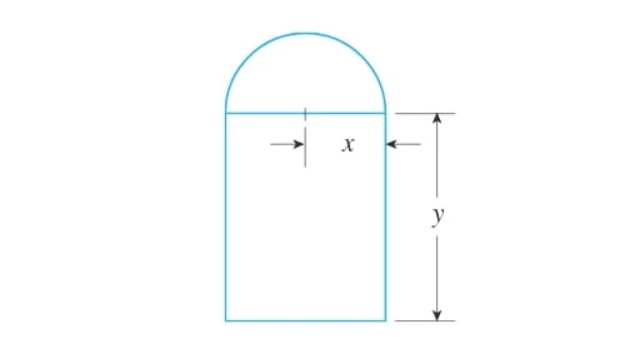
\includegraphics[width=0.5\textwidth]{NormanWindow.png}
    \caption{Picture of a Norman Window}
    \label{fig:my_image}
\end{figure}
\vspace{12cm}



To receive full credit, make sure to fully justify why the numbers you've found maximize the area. 

You are required to use a method we've learned in our course, such as the first derivative test, the second derivative test, the close interval method, or the first derivative test for absolute extrema, as a part of your justification. In addition, you need to make sure the method you use is suitable for the question.

%%%%%%%%%%%%%%%%%%%%%%%%%%%%%%%%%%%%%%%%%%%%%%%%%%%%%
%%%%%%%%%%% END PROBLEM A3 %%%%%%%%%%%%%%%%%%%%%%%%%%
%%%%%%%%%%%%%%%%%%%%%%%%%%%%%%%%%%%%%%%%%%%%%%%%%%%%%

\newpage

%%%%%%%%%%%%%%%%%%%%%%%%%%%%%%%%%%%%%%%%%%%%%%%%%%%%%
%%%%%%%%%%% BEGIN PROBLEM I1 %%%%%%%%%%%%%%%%%%%%%%%%
%%%%%%%%%%%%%%%%%%%%%%%%%%%%%%%%%%%%%%%%%%%%%%%%%%%%%

\item Suppose $v(t)$ represents the velocity (in meters per second) of a particle moving along a straight line at time $t$ (in seconds), for $0 \leq t \leq 6$.

\begin{enumerate}

\item[(a)] What are the units of $\displaystyle \int_1^4 v(t)\,dt$?  

\vspace{4cm}

\item[(b)] Let $s(t)$ represent the position of the particle at time $t$, and assume that $s'(t) = v(t)$.  

Explain what the quantity
\[
\int_1^4 v(t)\,dt
\]
represents in terms of $s(t)$. Be sure to include all units.

\vspace{4cm}

\item[(c)] Suppose the particle reaches its absolute minimum position at $t = 2$.  
Determine which of the following integrals must be positive. Select all that apply.

\[
\text{(i)}\ \int_0^2 v(t)\,dt 
\qquad
\text{(ii)}\ \int_2^5 v(t)\,dt
\qquad
\text{(iii)}\ \int_0^5 v(t)\,dt
\qquad
\text{(iv)}\ \int_5^2 v(t)\,dt
\]

\vspace{2cm}

\item[(d)] Suppose $\displaystyle \int_0^6 v(t)\,dt = 0$.  
What does this tell you about the position of the particle at $t=6$ compared to its position at $t=0$?  
Explain your reasoning.

\end{enumerate}


%%%%%%%%%%%%%%%%%%%%%%%%%%%%%%%%%%%%%%%%%%%%%%%%%%%%%
%%%%%%%%%%% END PROBLEM I1 %%%%%%%%%%%%%%%%%%%%%%%%%%
%%%%%%%%%%%%%%%%%%%%%%%%%%%%%%%%%%%%%%%%%%%%%%%%%%%%%

\newpage

%%%%%%%%%%%%%%%%%%%%%%%%%%%%%%%%%%%%%%%%%%%%%%%%%%%%%
%%%%%%%%%%% BEGIN PROBLEM I2 %%%%%%%%%%%%%%%%%%%%%%%%
%%%%%%%%%%%%%%%%%%%%%%%%%%%%%%%%%%%%%%%%%%%%%%%%%%%%%

\item The acceleration of a car along a straight track is described by the function $a(t)$, measured in meters per second squared, where $t$ is the time in seconds. The graph of $a(t)$ is given below.

\begin{center}
    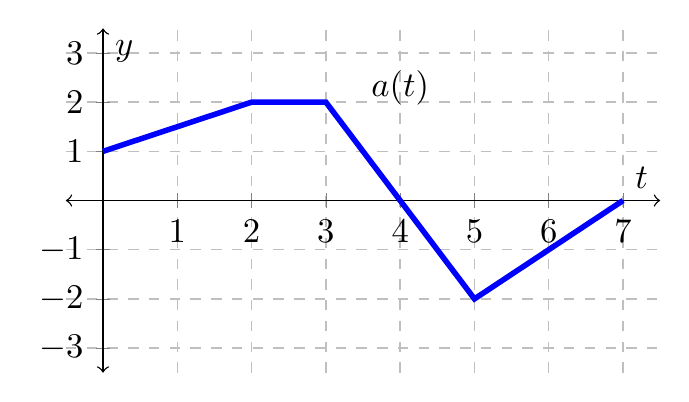
\begin{tikzpicture}[scale=1.25]
          \begin{axis}[
            xlabel={$t$},
            xtick={0,1,2,3,4,5,6,7,8},
            xticklabels={$0$,$1$,$2$,$3$,$4$,$5$,$6$,$7$},
            ytick={-3,-2,-1,0,1,2,3},
            yticklabels={$-3$,$-2$,$-1$,$0$,$1$,$2$,$3$},
            samples=320,
            domain=-0.5:7.5,
            restrict y to domain=-3.5:3.5,
            xmin=-0.5, xmax=7.5,
            ymin=-3.5, ymax=3.5,
            height=2in, width=3in,
            grid=both, grid style=dashed
          ]
          \draw[ultra thick, blue, -] (0,1) -- (2,2) -- (3,2) -- (5,-2) -- (7,0);
          \node at (4,2.3) {$a(t)$};
          \end{axis}
    \end{tikzpicture}
\end{center}

Use the properties of definite integrals (linearity, reversing limits, and interval addition) to answer the following questions. Show all work and clearly indicate where you have used any property of integration.

\begin{enumerate}

\item Find $\displaystyle \int_0^3 a(t)\,dt$.  

\vfill

\item Find $\displaystyle \int_3^5 a(t)\,dt$.  

\vfill

\item Suppose it is known that $\displaystyle \int_{3}^{-1} a(t)\,dt = 4$.  
Find the value of $\displaystyle \int_{-1}^{0} a(t)\,dt$.  

\vfill

\end{enumerate}

%%%%%%%%%%%%%%%%%%%%%%%%%%%%%%%%%%%%%%%%%%%%%%%%%%%%%
%%%%%%%%%%% END PROBLEM I2 %%%%%%%%%%%%%%%%%%%%%%%%%%
%%%%%%%%%%%%%%%%%%%%%%%%%%%%%%%%%%%%%%%%%%%%%%%%%%%%%

\newpage

\begin{center}
{\bf DO NOT REMOVE THIS SHEET FROM YOUR EXAM PACKET}
\end{center}

\begin{center}
    \begin{tabular}{ r | c | l }
    {\bf Description} & {\bf Formula} & {\bf Variables}\\
    perimeter of a semicircle & $P = \pi r$ & $r$ radius\\
    \hline
    area of a square & $A=s^2$ & $s=$ side length\\
    \hline
    area of a rectangle & $A=lw$ & $l=$ length, $w=$ width\\
    \hline
    perimeter of a rectangle & $P=2l + 2w$ & $l=$ length, $w=$ width\\
    \hline
    area of a triangle & $A=\frac12bh$ & $b=$ base, $h=$ height\\
    \hline
    area of a circle & $A=\pi r^2$ & $r=$ radius\\
    \hline
    area of a semicircle & $A=\frac{\pi r^2}{2}$ & $r=$ radius\\
    \hline
    volume of a rectangular box & $V=lwh$ & $l=$ length, $w=$ width, $h=$ height\\
    \hline
    %volume of a circular cylinder & $V=\pi r^2 h$ & $r=$ radius, $h=$ height\\
    %\hline
    %volume of a sphere & $V=\frac43\pi r^3$ & $r=$ radius\\
    %\hline
    revenue & $R(x) = p\cdot x = p\cdot Q$ & $p=$ unit price, $x=Q=$ quantity sold\\
    \hline
    profit & $P(x) = R(x) - C(x)$ & $R(x)=$ revenue, $C(x)=$ cost\\
    \hline
    average cost & $\overline C(x) = \frac{C(x)}{x}$ & $C(x)=$ cost\\
    \end{tabular}
\end{center}

\begin{center}
{\bf DO NOT REMOVE THIS SHEET FROM YOUR EXAM PACKET}
\end{center}

\newpage

This page is left blank intentionally.\\

Use this page if you need additional space to write your solutions to any problem. \\

If you wish this page graded, you must refer to this page on \textbf{the original page} of the problem. Otherwise, your grader will NOT consider your work on this page.

\end{enumerate}

\end{document}